% Created by tikzDevice version 0.10.1 on 2017-02-27 14:38:35
% !TEX encoding = UTF-8 Unicode
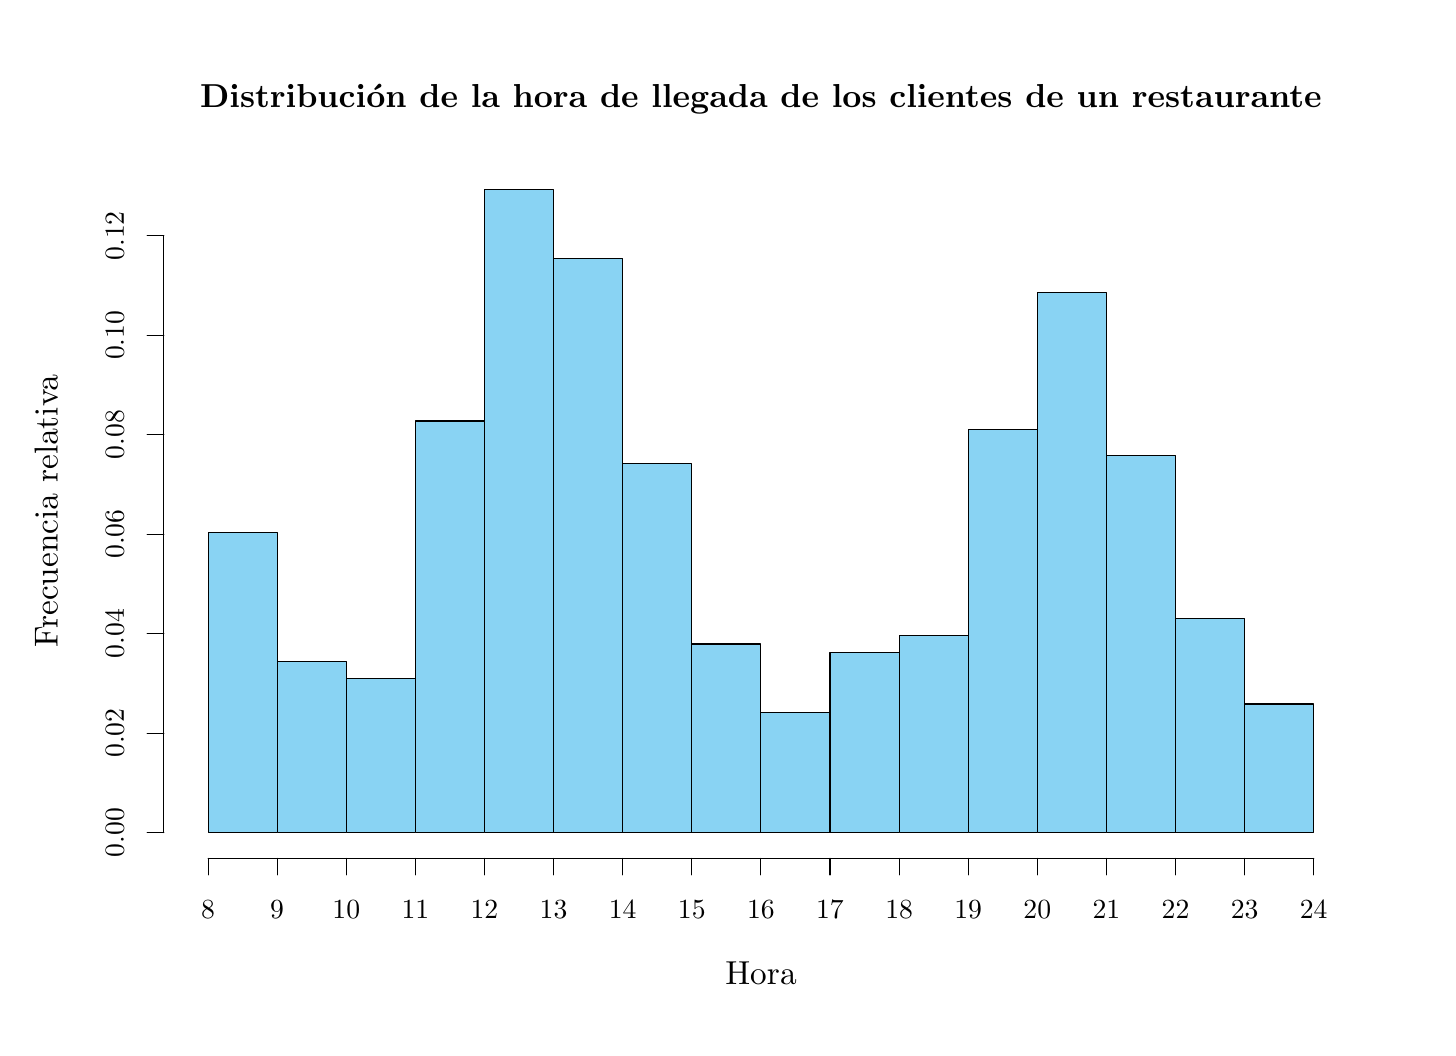
\begin{tikzpicture}[x=1pt,y=1pt]
\definecolor{fillColor}{RGB}{255,255,255}
\path[use as bounding box,fill=fillColor,fill opacity=0.00] (0,0) rectangle (505.89,361.35);
\begin{scope}
\path[clip] (  0.00,  0.00) rectangle (505.89,361.35);
\definecolor{drawColor}{RGB}{0,0,0}

\node[text=drawColor,anchor=base,inner sep=0pt, outer sep=0pt, scale=  1.20] at (264.94,332.61) {\bfseries Distribución de la hora de llegada de los clientes de un restaurante};

\node[text=drawColor,anchor=base,inner sep=0pt, outer sep=0pt, scale=  1.20] at (264.94, 15.60) {Hora};

\node[text=drawColor,rotate= 90.00,anchor=base,inner sep=0pt, outer sep=0pt, scale=  1.20] at ( 10.80,186.67) {Frecuencia relativa};
\end{scope}
\begin{scope}
\path[clip] (  0.00,  0.00) rectangle (505.89,361.35);
\definecolor{drawColor}{RGB}{0,0,0}

\path[draw=drawColor,line width= 0.4pt,line join=round,line cap=round] ( 49.20, 70.49) -- ( 49.20,286.13);

\path[draw=drawColor,line width= 0.4pt,line join=round,line cap=round] ( 49.20, 70.49) -- ( 43.20, 70.49);

\path[draw=drawColor,line width= 0.4pt,line join=round,line cap=round] ( 49.20,106.43) -- ( 43.20,106.43);

\path[draw=drawColor,line width= 0.4pt,line join=round,line cap=round] ( 49.20,142.37) -- ( 43.20,142.37);

\path[draw=drawColor,line width= 0.4pt,line join=round,line cap=round] ( 49.20,178.31) -- ( 43.20,178.31);

\path[draw=drawColor,line width= 0.4pt,line join=round,line cap=round] ( 49.20,214.25) -- ( 43.20,214.25);

\path[draw=drawColor,line width= 0.4pt,line join=round,line cap=round] ( 49.20,250.19) -- ( 43.20,250.19);

\path[draw=drawColor,line width= 0.4pt,line join=round,line cap=round] ( 49.20,286.13) -- ( 43.20,286.13);

\node[text=drawColor,rotate= 90.00,anchor=base,inner sep=0pt, outer sep=0pt, scale=  1.00] at ( 34.80, 70.49) {0.00};

\node[text=drawColor,rotate= 90.00,anchor=base,inner sep=0pt, outer sep=0pt, scale=  1.00] at ( 34.80,106.43) {0.02};

\node[text=drawColor,rotate= 90.00,anchor=base,inner sep=0pt, outer sep=0pt, scale=  1.00] at ( 34.80,142.37) {0.04};

\node[text=drawColor,rotate= 90.00,anchor=base,inner sep=0pt, outer sep=0pt, scale=  1.00] at ( 34.80,178.31) {0.06};

\node[text=drawColor,rotate= 90.00,anchor=base,inner sep=0pt, outer sep=0pt, scale=  1.00] at ( 34.80,214.25) {0.08};

\node[text=drawColor,rotate= 90.00,anchor=base,inner sep=0pt, outer sep=0pt, scale=  1.00] at ( 34.80,250.19) {0.10};

\node[text=drawColor,rotate= 90.00,anchor=base,inner sep=0pt, outer sep=0pt, scale=  1.00] at ( 34.80,286.13) {0.12};
\end{scope}
\begin{scope}
\path[clip] ( 49.20, 61.20) rectangle (480.69,312.15);
\definecolor{drawColor}{RGB}{0,0,0}
\definecolor{fillColor}{RGB}{137,211,243}

\path[draw=drawColor,line width= 0.4pt,line join=round,line cap=round,fill=fillColor] ( 65.18, 70.49) rectangle ( 90.15,178.93);

\path[draw=drawColor,line width= 0.4pt,line join=round,line cap=round,fill=fillColor] ( 90.15, 70.49) rectangle (115.12,132.46);

\path[draw=drawColor,line width= 0.4pt,line join=round,line cap=round,fill=fillColor] (115.12, 70.49) rectangle (140.09,126.26);

\path[draw=drawColor,line width= 0.4pt,line join=round,line cap=round,fill=fillColor] (140.09, 70.49) rectangle (165.06,219.21);

\path[draw=drawColor,line width= 0.4pt,line join=round,line cap=round,fill=fillColor] (165.06, 70.49) rectangle (190.03,302.86);

\path[draw=drawColor,line width= 0.4pt,line join=round,line cap=round,fill=fillColor] (190.03, 70.49) rectangle (215.00,278.07);

\path[draw=drawColor,line width= 0.4pt,line join=round,line cap=round,fill=fillColor] (215.00, 70.49) rectangle (239.97,203.71);

\path[draw=drawColor,line width= 0.4pt,line join=round,line cap=round,fill=fillColor] (239.97, 70.49) rectangle (264.94,138.65);

\path[draw=drawColor,line width= 0.4pt,line join=round,line cap=round,fill=fillColor] (264.94, 70.49) rectangle (289.92,113.87);

\path[draw=drawColor,line width= 0.4pt,line join=round,line cap=round,fill=fillColor] (289.92, 70.49) rectangle (314.89,135.56);

\path[draw=drawColor,line width= 0.4pt,line join=round,line cap=round,fill=fillColor] (314.89, 70.49) rectangle (339.86,141.75);

\path[draw=drawColor,line width= 0.4pt,line join=round,line cap=round,fill=fillColor] (339.86, 70.49) rectangle (364.83,216.11);

\path[draw=drawColor,line width= 0.4pt,line join=round,line cap=round,fill=fillColor] (364.83, 70.49) rectangle (389.80,265.68);

\path[draw=drawColor,line width= 0.4pt,line join=round,line cap=round,fill=fillColor] (389.80, 70.49) rectangle (414.77,206.81);

\path[draw=drawColor,line width= 0.4pt,line join=round,line cap=round,fill=fillColor] (414.77, 70.49) rectangle (439.74,147.95);

\path[draw=drawColor,line width= 0.4pt,line join=round,line cap=round,fill=fillColor] (439.74, 70.49) rectangle (464.71,116.97);
\end{scope}
\begin{scope}
\path[clip] (  0.00,  0.00) rectangle (505.89,361.35);
\definecolor{drawColor}{RGB}{0,0,0}

\path[draw=drawColor,line width= 0.4pt,line join=round,line cap=round] ( 65.18, 61.20) -- (464.71, 61.20);

\path[draw=drawColor,line width= 0.4pt,line join=round,line cap=round] ( 65.18, 61.20) -- ( 65.18, 55.20);

\path[draw=drawColor,line width= 0.4pt,line join=round,line cap=round] ( 90.15, 61.20) -- ( 90.15, 55.20);

\path[draw=drawColor,line width= 0.4pt,line join=round,line cap=round] (115.12, 61.20) -- (115.12, 55.20);

\path[draw=drawColor,line width= 0.4pt,line join=round,line cap=round] (140.09, 61.20) -- (140.09, 55.20);

\path[draw=drawColor,line width= 0.4pt,line join=round,line cap=round] (165.06, 61.20) -- (165.06, 55.20);

\path[draw=drawColor,line width= 0.4pt,line join=round,line cap=round] (190.03, 61.20) -- (190.03, 55.20);

\path[draw=drawColor,line width= 0.4pt,line join=round,line cap=round] (215.00, 61.20) -- (215.00, 55.20);

\path[draw=drawColor,line width= 0.4pt,line join=round,line cap=round] (239.97, 61.20) -- (239.97, 55.20);

\path[draw=drawColor,line width= 0.4pt,line join=round,line cap=round] (264.94, 61.20) -- (264.94, 55.20);

\path[draw=drawColor,line width= 0.4pt,line join=round,line cap=round] (289.92, 61.20) -- (289.92, 55.20);

\path[draw=drawColor,line width= 0.4pt,line join=round,line cap=round] (314.89, 61.20) -- (314.89, 55.20);

\path[draw=drawColor,line width= 0.4pt,line join=round,line cap=round] (339.86, 61.20) -- (339.86, 55.20);

\path[draw=drawColor,line width= 0.4pt,line join=round,line cap=round] (364.83, 61.20) -- (364.83, 55.20);

\path[draw=drawColor,line width= 0.4pt,line join=round,line cap=round] (389.80, 61.20) -- (389.80, 55.20);

\path[draw=drawColor,line width= 0.4pt,line join=round,line cap=round] (414.77, 61.20) -- (414.77, 55.20);

\path[draw=drawColor,line width= 0.4pt,line join=round,line cap=round] (439.74, 61.20) -- (439.74, 55.20);

\path[draw=drawColor,line width= 0.4pt,line join=round,line cap=round] (464.71, 61.20) -- (464.71, 55.20);

\node[text=drawColor,anchor=base,inner sep=0pt, outer sep=0pt, scale=  1.00] at ( 65.18, 39.60) {8};

\node[text=drawColor,anchor=base,inner sep=0pt, outer sep=0pt, scale=  1.00] at ( 90.15, 39.60) {9};

\node[text=drawColor,anchor=base,inner sep=0pt, outer sep=0pt, scale=  1.00] at (115.12, 39.60) {10};

\node[text=drawColor,anchor=base,inner sep=0pt, outer sep=0pt, scale=  1.00] at (140.09, 39.60) {11};

\node[text=drawColor,anchor=base,inner sep=0pt, outer sep=0pt, scale=  1.00] at (165.06, 39.60) {12};

\node[text=drawColor,anchor=base,inner sep=0pt, outer sep=0pt, scale=  1.00] at (190.03, 39.60) {13};

\node[text=drawColor,anchor=base,inner sep=0pt, outer sep=0pt, scale=  1.00] at (215.00, 39.60) {14};

\node[text=drawColor,anchor=base,inner sep=0pt, outer sep=0pt, scale=  1.00] at (239.97, 39.60) {15};

\node[text=drawColor,anchor=base,inner sep=0pt, outer sep=0pt, scale=  1.00] at (264.94, 39.60) {16};

\node[text=drawColor,anchor=base,inner sep=0pt, outer sep=0pt, scale=  1.00] at (289.92, 39.60) {17};

\node[text=drawColor,anchor=base,inner sep=0pt, outer sep=0pt, scale=  1.00] at (314.89, 39.60) {18};

\node[text=drawColor,anchor=base,inner sep=0pt, outer sep=0pt, scale=  1.00] at (339.86, 39.60) {19};

\node[text=drawColor,anchor=base,inner sep=0pt, outer sep=0pt, scale=  1.00] at (364.83, 39.60) {20};

\node[text=drawColor,anchor=base,inner sep=0pt, outer sep=0pt, scale=  1.00] at (389.80, 39.60) {21};

\node[text=drawColor,anchor=base,inner sep=0pt, outer sep=0pt, scale=  1.00] at (414.77, 39.60) {22};

\node[text=drawColor,anchor=base,inner sep=0pt, outer sep=0pt, scale=  1.00] at (439.74, 39.60) {23};

\node[text=drawColor,anchor=base,inner sep=0pt, outer sep=0pt, scale=  1.00] at (464.71, 39.60) {24};
\end{scope}
\end{tikzpicture}
